\documentclass[11pt,addpoints,answers]{exam}

\usepackage{amssymb,amsmath,amsthm,amsfonts,mathtools,dsfont,thmtools}
\usepackage{suffix}
\usepackage{natbib} 
\usepackage{csquotes} 
\usepackage{subcaption}
\usepackage[inline]{enumitem} 
\usepackage{booktabs}
\usepackage[usenames,dvipsnames]{xcolor}
\usepackage{wrapfig}
\usepackage{hyperref}
\usepackage[capitalize,noabbrev]{cleveref}
\hypersetup{
  colorlinks=true,
  linkcolor=RawSienna,
  urlcolor=Cyan,
  citecolor=gray
}

\setlength{\parskip}{6pt}
\setlength{\parindent}{0pt}
\setlength{\headheight}{14pt}
\usepackage{listings}
\usepackage{adjustbox}

\chead{EN.601.475/675 Machine Learning}
\date{}
\pagestyle{headandfoot}
\begin{document}
\thispagestyle{headandfoot}

\begin{center}
  {\Large \bf{Homework 2: Due \textbf{October 3rd, 11:59pm ET}}}
\end{center}

\qformat{\textbf{\Large Question \thequestion\ \dotfill \emph{\totalpoints\ points}}}

\begin{center}
\fbox{\fbox{\parbox{6.5in}{
\textbf{Submission Instructions:} You will upload your solutions to the analytical portion and the programming portion separately to Gradescope.  
\begin{itemize}
\item \textbf{Analytical Part (this file)}: You should use LaTeX to type up your solutions (e.g., via Overleaf or similar), but please ensure that \textbf{each part (e.g., a, b, etc) begins on a new page} (to facilitate grading in Gradescope). You will upload the PDF to the assignment ``Homework 2: Analytical'' on Gradescope.
\item \textbf{Programming Part (see Canvas)}: You should upload your \texttt{.ipynb} file directly to Gradescope under the assignment ``Homework 2: Programming''.
\end{itemize}
Note that you must upload \textbf{both} parts to their respective assignments on Gradescope.
\vspace{0.1in}

\textbf{Collaboration Policy:} You may work with other students on the homework assignments, but you must write up and submit your own work independently, and you must acknowledge your collaborators on the first page of your homework submission.
\vspace{0.1in}

\textbf{Late Submission Policy:} You have up to 48 hours of ``slack'' for late submissions of homework assignments, across \textbf{all} homework assignments.  Once you have exhausted your budget, we will deduct points for late submissions.  However, \textbf{no individual assignment may be submitted more than 48 hours late}, as we will release solutions at this time.
\vspace{0.1in}

\textbf{Use of Generative AI:} You are \textbf{not permitted} to use generative AI tools (e.g., ChatGPT) for problems on this problem set.
}}}
\end{center}

% TODO: Type out your name and email in these spaces, replacing the \enspace\hrulefill
\makebox[\textwidth]{Name:\enspace Rashed Aldulijan\hrulefill}\vspace{0.2in}
\makebox[\textwidth]{JHU Email:\enspace ralduli1@jh.edu\hrulefill}\vspace{0.2in}
\makebox[\textwidth]{Collaborators (or \enquote{None}):\enspace None\hrulefill}

\begin{center}
The analytical portion (this file) of HW1 has \numquestions\ questions, for a total of \numpoints\
points.
\end{center}

\newpage

\section*{Part 1: Analytical Questions}

\begin{questions}
\question%
Consider the logistic regression classification problem, where our data is given by the following two points
\begin{align*}
  x_1 &= -1 & y_1 &= 0 \\
  x_2 &= 1 & y_2 &= 1
\end{align*}
Let our logistic regression model be given by the following
\begin{equation}
  P(Y = 1 \mid X = x) = \frac{\exp(\beta x)}{1 + \exp(\beta x)}
\end{equation}
\begin{parts}
\part[5]%
Show that the log-likelihood of the data is given by 
\begin{equation}
L(\beta) = - \log (1 + \exp(-\beta)) + \beta - \log (1 + \exp(\beta))
\end{equation}
\begin{solutionorbox}
  \[ P(y = 1 | x = 1) = \frac{exp(\beta)}{1 + exp(\beta)} \]
  \[ P(y = 0 | x = -1) = \frac{1}{1 + exp(-\beta)} \]
  \[ L(\beta) = log(P(y = 1 | x = 1)) + log(P(y = 0 | x = -1)) \]
  \[ L(\beta) = \beta - log(1 + exp(\beta)) - log(1+exp(-\beta)) \]
\end{solutionorbox}
\newpage
\part[5]%
Show that the derivative of the log-likelihood is equal to 
\begin{equation}
\frac{\partial L(\beta)}{\partial \beta} = 1 - \frac{\exp(\beta)}{1 + \exp(\beta)} + \frac{\exp(-\beta))}{1 + \exp(-\beta)} 
\end{equation}
\begin{solutionorbox}
  using the log-likelihood from part (a):
  \[ L(\beta) = - log(1 + exp(-\beta)) + \beta - log(1 + exp(\beta)) \]
  \[ \frac{\partial L(\beta)}{\partial \beta} = \frac{exp(-\beta)}{1 + exp(-\beta)} + 1 - \frac{exp(\beta)}{1 + exp(\beta)} \]
  \[ \frac{\partial L(\beta)}{\partial \beta} = 1 - \frac{exp(\beta)}{1 + exp(\beta)} + \frac{exp(-\beta)}{1 + exp(-\beta)} \]
\end{solutionorbox}
\newpage
\part[5]%
Argue that the derivative from the previous part is always strictly greater than zero, regardless of the value of $\beta$.
\begin{solutionorbox}
  \[ \frac{\partial L(\beta)}{\partial \beta} = 1 - \frac{exp(\beta)}{1 + exp(\beta)} + \frac{exp(-\beta)}{1 + exp(-\beta)} \]
  \[ = 1 - \frac{exp(\beta)}{1 + exp(\beta)} + \frac{1}{exp(\beta) + 1} \]
  \[ = \frac{exp(\beta) + 1 - \exp(\beta) + 1}{exp(\beta) + 1} \]
  \[ \boxed{= \frac{2}{exp(\beta) + 1} > 0} \]
\end{solutionorbox}
\newpage
\part[5]%
As a result, there is no optimal solution $\beta$, but rather, for any $\beta_1, \beta_2$ where $\beta_1 < \beta_2$, the likelihood will be greater under $\beta_2$.  Provide some brief intuition (one or two sentences) as to why this behavior makes sense.
\begin{solutionorbox}
  The derivative of the log-likelihood is always positive, meaning that the log-likelihood is always increasing as beta increases. Therefore, there is no maximum value for beta, and the likelihood will always be greater for larger values of beta.
\end{solutionorbox}

\newpage
\part[5] Explain how it is possible that both (a) no optimal solution for $\beta$ exists for this data, and (b) the logistic regression likelihood is concave (and hence, minimizing the negative log likelihood is a convex optimization problem).
\begin{solutionorbox}
  (a) There is no \textbf{finit} optimal solution for this data because the derivative can not equal to zero, which mean there is no exact horizental line on the function. (b) However, because logistic regression is concave in every parameter, its limit of the weights tends to go to infinity because it cannot be exactly horizental, but the derivative line can be approximatly horizental, so it can be solved using approximations methods like gradient descent.
\end{solutionorbox}

\end{parts}
\textbf{Coda:} This is an example of a `linearly separable' problem, where there exists a linear decision-boundary (in this case, any threshold between $-1, 1$) such that all of our positive examples lie on one side of the decision-boundary, and all negative examples lie on the other side.  It is worth knowing that logistic regression will (in general) exhibit this type of behavior on linearly separable data.

\newpage
\question%
Consider minimizing the following simple quadratic function.
\begin{equation*}
f(\beta) = \beta^2
\end{equation*}
Clearly, the minimizer is $\beta = 0$, but we will use this problem to illustrate the use of \textit{local search} methods, and their performance at finding this solution. You consider two methods for optimizing this function by iteratively updating your guess for the minimizer:
\begin{itemize}
  \item Newton-Raphson Method: $\beta_t = \beta_{t-1} - f'(\beta_{t-1}) / f''(\beta_{t-1})$
  \item Gradient Descent: $\beta_t = \beta_{t-1} - \eta f'(\beta_{t-1})$ for some $\eta > 0$
\end{itemize}

\begin{parts}

\part[5]%
For any initial value of $\beta_0$, what is the value of $\beta_1$, the revised guess after one iteration, for the Newton-Raphson method?  How does this guess depend on $\beta_0$?
\begin{solutionorbox}
  \[ \beta_1 = \beta_0 - \frac{2*\beta_0}{2} = 0\]
\end{solutionorbox}
\newpage

\part[5]%
For gradient descent, the behavior depends on our choice of the learning rate $\eta$.  Using $\eta = 1$, what is the value of $\beta_1$ after a single iteration?  How does this guess depend on $\beta_0$?  What will occur if you continue to iteratively update in this fashion?
\begin{solutionorbox}
  \[ \beta_1 = \beta_0 - (1)2\beta_0 \]
  \[ \beta_1 = -\beta_0 \]
  This learning rate is to big, the betas will be updated between the negative and positive of the same number infinitly.
\end{solutionorbox}
\newpage

\part[5]%
Similar to the previous question, give the value of $\beta_1$ in terms of $\beta_0$ for the step sizes $\eta = 1/4$ and $\eta = 4$.  Interpret in a sentence or two what will occur if you run gradient descent under each of these step sizes. Why is $\eta = 1/4$ a better choice for this problem?
\begin{solutionorbox}
  \[ \beta_1 = \beta_0 - (1/4)2\beta_0 \]
  \[ \boxed{\beta_1 = \frac{1}{2}\beta_0} \]
  \[ \beta_1 = \beta_0 - (4)2\beta_0 \]
  \[ \boxed{\beta_1 = -7\beta_0} \]
  If we use $\eta = 1/4$, the betas will converge to zero, but if we use $\eta = 4$, the betas will diverge to infinity. $\eta = 1/4$ is a better choice because it converges to zero.
\end{solutionorbox}

\end{parts}

\newpage
\question%

\textbf{Complex Models with Linear Pieces:}

Every Monday, Blue Jay Brian heads to Hopkins Café for lunch around noon. To his frustration, sometimes the line is short and manageable, while other times the wait seems to explode. Determined to get to the bottom of this mystery (and maybe plan his lunch better), Brian decides to conduct a small study of the café wait times.

He records the average wait time (in minutes) at several time points between 11:40am and 12:00pm. To keep things simple, Brain defines
\[
t = \text{minutes since 11:40am},
\]
so that $t=0$ corresponds to 11:40 and $t=20$ corresponds to 12:00.

The data Brian collected are shown below:

\[
\begin{array}{c|c|c|c}
\text{Time} & t & \text{Wait (min)} \\
\hline
11{:}40 & 0 & 1.0 \\
11{:}45 & 5 & 1.6 \\
11{:}48 & 8 & 1.8 \\
11{:}51 & 11 & 3.0 \\
11{:}54 & 14 & 6.0 \\
12{:}00 & 20 & 12.0 \\
\end{array}
\]

\begin{figure}[!h]
    \centering
    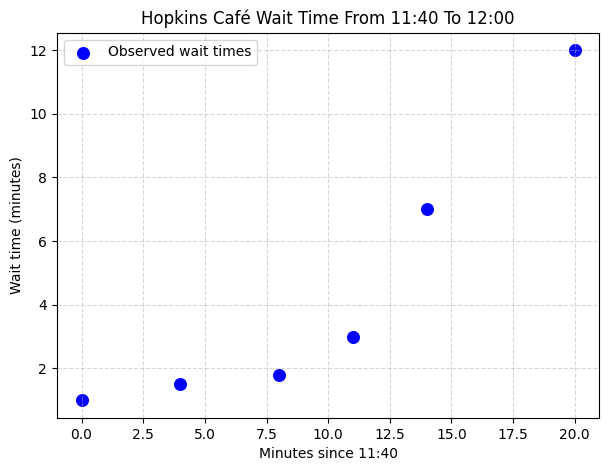
\includegraphics[width=0.65\linewidth]{figure_1.png}
    \label{fig:placeholder}
\end{figure}

As a first attempt, Brian tries a simple linear regression model:
\[
\text{Wait}(t) = \beta_0 + \beta_1 t + \varepsilon
\]

\newpage
\begin{parts}
  \part[6]%
  Following lecture notation, let $\tilde X$ denote the input matrix with a leading column of ones (for the intercept). Write down the explicit form of $\tilde X$ and the output vector $y$ for Brian's data.
  Then, give the closed-form expression for the least squares solution $\vec{\beta}$ in terms of $\tilde X$ and $y$ (do not compute the numerical values). State the dimension of $\vec{\beta}$ for this problem.
  
  \begin{solutionorbox}[2in]
    Your solution goes here.  \LaTeX\ tip: You can use this code to write a matrix
    \begin{equation}
      A = \begin{bmatrix} 
        a_1 & a_2 \\ 
        a_3 & a_4 \\ 
    \end{bmatrix}  
  \end{equation}
  \begin{equation}
    \tilde{X}=\begin{bmatrix} 
      1 & 0 \\ 
      1 & 5 \\ 
      1 & 8 \\ 
      1 & 11 \\ 
      1 & 14 \\ 
      1 & 20 \\ 
    \end{bmatrix}
  \end{equation}
  \begin{equation}
    y=\begin{bmatrix}
      1.0 \\
      1.6 \\
      1.8 \\
      3.0 \\
      6.0 \\
      12.0 \\
    \end{bmatrix}
  \end{equation}
  \[ \vec{\beta} = (\tilde{X}^T\tilde{X})^{-1}\tilde{X}^Ty \]
  \[ \text{dim}(\vec{\beta}) = 2 by 1 \]
  \end{solutionorbox}

  \newpage
After fitting the simple linear regression, Brian checks the differences between the observed wait times and the fitted values. See plot next page.

\begin{figure}[!h]
    \centering
    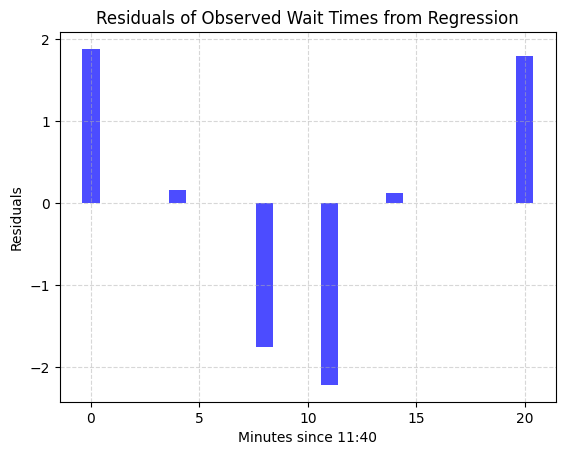
\includegraphics[width=0.65\linewidth]{figure_2.png}
    \label{fig:residuals}
\end{figure}

Notice how the residuals are not randomly scattered around zero. This suggests that a single straight line may not be flexible enough.

  \part[6]%
  Propose a two-piece linear model for Brian's data, where the slope of the line changes at $t=10$ (i.e., 11:50am). Require the two pieces connect at $t=10$ (no sudden jump in predicted wait time).
  Write down the regression equation in terms of $\beta_0, \beta_1, \beta_2$ and the indicator feature
  \[
  h(t) =
  \begin{cases}
    0 & t \leq 10, \\
    1 & t > 10.
  \end{cases}
  \]

  \begin{solutionorbox}[2in]
    \[ \hat{y} = \beta_0 + \beta_1\hat{X} + \beta_2(\hat{X} - 10)h(t) \]
    \[ \hat{y} = \beta_0 + \beta_1\hat{X} + \beta_2\hat{X}^* \]
    where \[ \hat{X}^* = (\hat{X} - 10)h(t) \]
  \end{solutionorbox}

  \newpage
  \part[8]%
  The model in part (b) should introduce one additional feature.
  Following the same approach as in part (a), write down the input matrix $\tilde X$ for the two-piece model. (Note: you do not need to rewrite $y$ or the closed-form solution; do not attempt to write separate closed forms for each piece.)
  \begin{solutionorbox}[3in]
    \[ \tilde{X}=\begin{bmatrix} 
      1 & 0 & 0 \\ 
      1 & 5 & 0 \\ 
      1 & 8 & 0 \\ 
      1 & 11 & 1 \\ 
      1 & 14 & 4 \\ 
      1 & 20 & 10 \\ 
    \end{bmatrix} \]
  \end{solutionorbox}

  \newpage
  \part[5]%
  Instead of adding more features as we do for parts (b)-(c), Brian considers modifying the output side of the model
  with a non-linear link function. For example, suppose he models
  \[
  \text{Wait}(t) = \exp(\beta_0 + \beta_1 t) + \varepsilon.
  \]
  Give one advantage \emph{or} one tradeoff of this exponential transformation compared
  to the two-piece linear model in parts (b)-(c).
  
  \begin{solutionorbox}[2.5in]
    exponential model would have a high variance on the training data, which would make it overfitting the data, and would do porely on the test data.
  \end{solutionorbox}
  
\end{parts}

\newpage

\question
A drug company wants to estimate the true effect \( \mu_i \) of a treatment for each patient group. Each group gives a noisy measurement:
\[
y_i \sim \mathcal{N}(\mu_i, \sigma^2)
\]

The company believes the \( \mu_i \)'s are similar, so it uses a \textbf{shrinkage estimator}:
\[
\hat{\mu}_i(\lambda) = (1 - \lambda)y_i + \lambda \bar{y}, \quad \text{where} \quad \bar{y} = \frac{1}{n} \sum_{j=1}^n y_j
\]

This pulls each estimate toward the global average. The shrinkage strength is controlled by \( \lambda \in [0, 1] \).

\begin{parts}
    \part[10] Compute the bias and variance of $\hat{\mu}_i(\lambda)$.

    \begin{solutionorbox}
      Variance:
      \[ Var(y_i) = \sigma^2 \]
      \[ Var(\bar{y}) = \frac{\sigma^2}{n} \]
      \[ Cov(y_i, \bar{y}) = E[(y_i - Ey_i)(\frac{1}{n}\sum_{j = 1}^{n}y_i - E(\frac{1}{n}\sum_{j = 1}^{n}y_i))]\]
      \[ = \frac{1}{n}\sum_{j=1}^{n} Cov(y_i,y_j) = \frac{1}{n} Var(y_i) = \boxed{\frac{1}{n}\sigma^2}\]
      \[ Var(\hat{\mu_i}(\lambda)) = Var((1-\lambda)y_i + \lambda\bar{y})\]
      \[ = (1-\lambda)^2 Var(y_i) + \lambda^2 Var(\bar{y}) + 2(1-\lambda)(\lambda)Cov(y_i, \bar{y}) \]
      \[ = \boxed{(1-\lambda)^2 \sigma^2 + \lambda^2 \frac{\sigma^2}{n} + \frac{2(1-\lambda)(\lambda)}{n} \sigma^2}\]
      Bias:
      \[ E[\hat{\mu_i}(\lambda)] = (1-\lambda) Ey_i + \lambda E\bar{y} \]
      \[ = (1 - \lambda) \mu_i\ + \lambda\bar{\mu} \]
      \[ Bias(\hat{\mu_i}(\lambda)) = E[(1 - \lambda)y_i + \lambda \bar{y}] - \mu_i\]
      \[ = (1 - \lambda) \mu_i\ + \lambda\bar{\mu} - \mu_i\]
      \[ = \lambda(\bar{\mu} - \mu_i)\]
    \end{solutionorbox}


    \newpage
    \part[10] Derive the expected squared error (also known as the risk) of the estimator $\hat{\mu}_i(\lambda)$, or $R(\hat{\mu}_i(\lambda)) = \mathbb{E}[(\hat{\mu}_i(\lambda) - \mu_i)^2]$, in terms of $\lambda$, $\mu_i$, $\bar{\mu}$, and $\sigma^2$. Then, interpret your result to explain how the bias-variance tradeoff depends on different values for $\lambda$.

    \begin{solutionorbox}
     \[ E[(\hat{\mu}_i(\lambda) - \mu_i)^2] = E[\hat{\mu}_i(\lambda)^2] - 2\mu_i E[\hat{\mu}_i(\lambda)] + \mu_i^2 \]
     \[ = Var(\hat{\mu}_i(\lambda)) + (E[\hat{\mu}_i(\lambda)])^2 - 2\mu_i E[\hat{\mu}_i(\lambda)] + \mu_i^2 \]
     \[ = Var(\hat{\mu}_i(\lambda)) + (E[\hat{\mu}_i(\lambda)] - \mu_i)^2 \]
     \[ = Var(\hat{\mu}_i(\lambda)) + Bias(\hat{\mu}_i(\lambda))^2 \]
     \[ = (1-\lambda)^2 \sigma^2 + \lambda^2 \frac{\sigma^2}{n} + \frac{2(1-\lambda)(\lambda)}{n} \sigma^2 + (\lambda(\bar{\mu} - \mu_i))^2 \]
     \[ = \boxed{(1-\lambda)^2 \sigma^2 + \lambda^2 \frac{\sigma^2}{n} + \frac{2(1-\lambda)(\lambda)}{n} \sigma^2 + \lambda^2(\bar{\mu} - \mu_i)^2} \]
      When we have too large lambda, the bias will be high and the variance will be low. When we have too small lambda, the bias will be low and the variance will be high. So we need to find a balance between bias and variance by choosing an appropriate value for lambda.     
     
    \end{solutionorbox}

    \newpage
        \part[10] Now assume that the true effects $\mu_i$ are random variables drawn from a prior distribution: $\mu_i \sim \mathcal{N}(0, \tau^2)$. Given the observation $y_i \sim \mathcal{N}(\mu_i, \sigma^2)$, derive the conditional posterior mean: $\mathbb{E}[\mu_i \mid y_i]$.

        \textit{Hint: Use the fact that the posterior is proportional to the product of the likelihood and the prior:
        $p(\mu_i \mid y_i) \propto \text{Likelihood} \times \text{Prior}$.}

        \begin{solutionorbox}
          \[ p(y_i | \mu_i) = \frac{1}{\sqrt{2\pi\sigma^2}} \int\exp\left(-\frac{(y_i - \mu_i)^2}{2\sigma^2}\right) dy_i\]
          \[ p(\mu_i) = \frac{1}{\sqrt{2\pi\tau^2}} \int\exp\left(-\frac{\mu_i^2}{2\tau^2}\right) d\mu_i\]
          \[ p(\mu_i | y_i) \propto p(y_i | \mu_i)p(\mu_i) \]
          \[ \propto \exp\left(-\frac{(y_i - \mu_i)^2}{2\sigma^2}\right)\exp\left(-\frac{\mu_i^2}{2\tau^2}\right) \]
          \[ \propto \exp\left(-\frac{1}{2}\left(\frac{(y_i - \mu_i)^2}{\sigma^2} + \frac{\mu_i^2}{\tau^2}\right)\right) \]
          \[ \propto \exp\left(-\frac{1}{2}\left(\mu_i^2(\frac{1}{\sigma^2} + \frac{1}{\tau^2}) - 2\mu_i\frac{y_i}{\sigma^2}\right)\right) \]
          \[ E[\mu_i | y_i] \text{ would be the mean of the above distribution }\]  
        \end{solutionorbox}

    \end{parts}

\newpage
\question% 
Suppose we train a model on a dataset $\mathcal{D}=\{(x_i,y_i)\}_{i=1}^n$. It tends to perform better on training data than on unseen data due to overfitting. Optimism formalizes this performance difference.

\begin{parts}
  \part[10]%
Assume the classical linear model here: \\
\[Y = X\beta + \varepsilon, \quad \varepsilon \sim \mathcal{{N}}(0, \sigma^2 I_n)\]\\
Where we let:
\begin{itemize}
    \item $X \in \mathbb{R}^{n \times d}$
    \item n be the number of data points
    \item d be the number of parameters in our model
    \item the least squares estimator be $\hat{\beta}=(X^\top X)^{-1} X^\top Y$
    \item the fitted values be $\hat{Y} = X(X^\top X)^{-1} X^\top Y$
\end{itemize}

Show that $\sum_{i=1}^n \text{Cov}(\hat{f}_D(x_i), Y_i) = d\sigma^2$\\
Hint: Let $H = X(X^\top X)^{-1} X^\top$. Use $\hat{f}_D(x_i) = \sum_{j=1}^n H_{ij}Y_j$, independence of noise, and the cyclic property of the trace (of a matrix), specifically that $\text{tr}(H) = \text{tr}(X^\top X (X^\top X)^{-1})$.  Recall also that $\text{Cov}(.)$ is an expectation, and thus obeys linearity of expectation, namely that $\mathbb{E}[a X + b Y]$ =
$a \mathbb{E}[X] + b \mathbb{E}[Y]$.
  \begin{solutionorbox}[2in]
    \[ \sum_{i=1}^{N} Cov(HY, Y) = \]
    \[ = \sum_{i=1}^{N}E[(HY-E(HY))(Y-EY)] \]
    \[ = \sum_{i=1}^{N}H*Cov(Y,Y) = \sum_{i=1}^{N}H*Var(Y) = \sum_{i=1}^{N}H\sigma^2 I_n \]
    \[ = \sigma^2 I_n*tr(H) = \sigma^2 I_n*tr((X^\top X (X^\top X)^{-1})) = \boxed{d\sigma^2}\]
  \end{solutionorbox}

  \newpage
  \part[5]%
  What is the expected optimism of this model? Explain why this result makes sense in terms of model complexity and overfitting?

  \begin{solutionorbox}[5in]
    According to The Elements of Statistical Learning by Hastie, Tibshirani, and Friedman.
    \[ op = Err_{in} - \overline{err} = \frac{2}{n}\sum_{i=1}^{n}Cov(\hat{y_i}, y_i) = \frac{2}{n}d\sigma^2 \]
    This result makes sense because as the number of parameters in the model increases, the model becomes more complex and is more likely to overfit the training data. This leads to a larger difference between the in-sample error and the test error, which is captured by the optimism.
  \end{solutionorbox}
  \end{parts}

\end{questions}

\newpage
\section*{Part 2: Programming Questions}

Be sure to complete the programming questions as well, and submit your final notebook on Gradescope.  Your PDF submission will focus on the questions above, while your notebook code will serve as your submission for the programming portion (questions can be found on Canvas).  This text is here just to remind you to submit the programming portion, and you may delete it when submitting your analytical solutions.

The link to the python notebook for Part 2 can be found here: \url{https://colab.research.google.com/drive/1PEWY8zdhHxoZ18lKHqkfx_1PucKluXDE?usp=sharing}

As noted in the notebook, \textbf{be sure to make your own copy of the notebook before doing anything else}.

\end{document}
